\documentclass[10pt,a4paper]{article}
\usepackage{graphicx}
\graphicspath{ {images/} }
\usepackage[utf8]{inputenc}
\usepackage{amsmath}
\usepackage{amsfonts}
\usepackage{amssymb}
\usepackage[left=2.5cm,right=2.5cm,top=2.5cm,bottom=2.5cm]{geometry}
\author{Sofía Mara Rivas Cuevas\\ Pablo Marcos Parra}

\title{PRACTICA 1. INFERENCIA ESTADISTICA II}
\begin{document}
\maketitle{}
\section{Enunciado de la practica}
Considerar una muestra aleatoria de tamaño n = 30 de una población cuya distribución es una mixtura de dos distribuciones exponenciales con funciones de densidad:\\
\\
\[f_{1}(x) = exp(-x)\]
\\
\[f_{2}(x) = 2exp(-2x)\]\\
\\
y proporciones p y 1-p respectivamente.Los datos observados son los siguientes:\\
\\
\\
y$\leftarrow$ c(0.92169370,0.20110924,0.08299092,1.27148296,0.08975299,2.49922718\\
\\
,4.34097682,0.39260263,0.06973844,0.05284850,0.40770048,0.03917915\\
\\
,0.19068404,1.26898667,0.53213247,0.52049674,0.22417266,0.18774498\\
\\
,0.16727780,0.44944121,1.10100809,0.84404590,0.66023800,2.86944266\\
\\
,0.08869227,0.85046707,0.41026355,0.28243983,0.07341746,0.10278472)\\
\\
\\
\\
\textbf{a)Obtener intervalos de confianza, de Wald, para p, con confianza 0.95.}\\
\\
\\
\textbf{b) Obtener el pvalor del test de razón de verosimilitud para contrastar la hipótesis nula, H0: p=0.5.}
\\
\\
\\
\textbf{c) Utilizar el algoritmo EM para aproximar el estimador máximo verosímil de p, utilizando el valor inicial 0.5 y 25 iteraciones.} 

\newpage
\section{APARTADO A)}

Para calcular el EMV de \textit{p} vamos a utilizar la función \texttt{optim} de R.\\
\\
La función de la mixtura es: $f(y_{i},p) = pf_{1}(y_{i}) + (1-p)f_{2}(y_{i})$\\
\\
La función de verosímilitud es: $L(p,y_{i})=$
$\displaystyle\prod_{i=1}^{n} pf_{1}(y_{i}) + (1-p)f_{2}(y_{i})
$\\
\\
\\
A la hora de pasarlo a R utilizamos la menos log-verosímilitud ( a partir de ahora la llamaremos mlv) y utilizando la función mencionada anteriormente calcularemos el EMV:\\

\begin{figure}[h]
	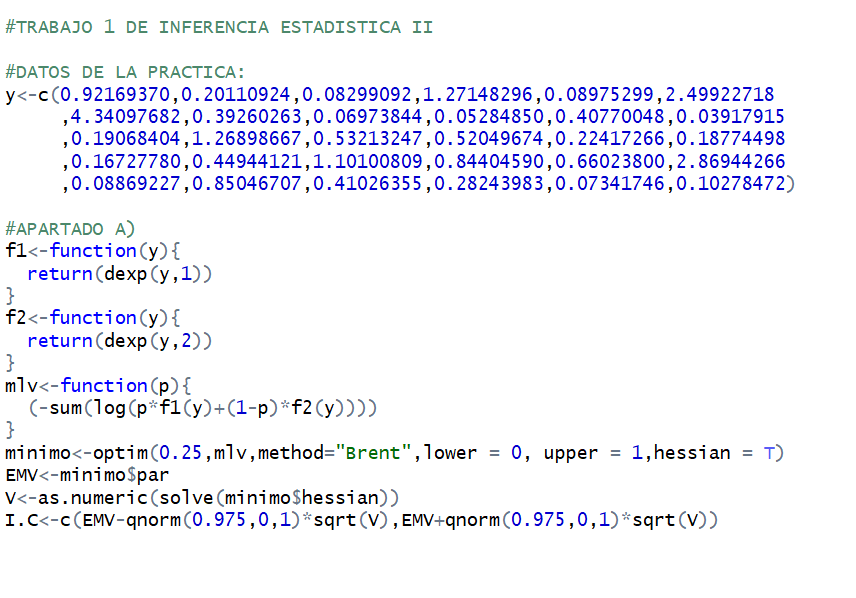
\includegraphics[width=13cm, height=9cm]{APARTADO A.PNG}
	\centering
\end{figure}
\begin{figure}[h]
	\fbox{EMV = 0.3658762}
	\centering
\end{figure}
\begin{figure}[h]
	\fbox{I.C de Wald = ( -0.08646918, 0.81822162 )}
	\centering
\end{figure}
La raíz de la varianza no está acotada y se nos puede ir a -$\infty$, como se trata de una proporción el intervalo tiene que estar entre 0 y 1.


\newpage
\section{APARTADO B} 
La razón de verosímilitud:
\begin{figure}[h]
	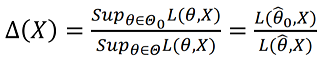
\includegraphics[scale=0.3]{razon de verosimilitud.PNG}
	\centering
\end{figure}\\
El estadístico razón de verosímilitud:\\
\begin{figure}[h]
	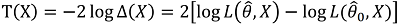
\includegraphics[scale=0.3]{estadistico.PNG}
	\centering
\end{figure}\\
En el siguiente fracmento de código está la solucion de este apartado:
\begin{figure}[h]
	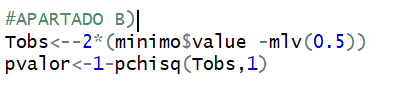
\includegraphics[scale=1]{apartadob.PNG}
	\centering
	\\
	\fbox{P-Valor = 0.583717}
	\centering
\end{figure}\\
\newpage
\section{APARTADO C}












\end{document}